%% This is file `elsarticle-template-1-num.tex',
%%
%% Copyright 2009 Elsevier Ltd
%%
%% This file is part of the 'Elsarticle Bundle'.
%% ---------------------------------------------
%%
%% It may be distributed under the conditions of the LaTeX Project Public
%% License, either version 1.2 of this license or (at your option) any
%% later version.  The latest version of this license is in
%%    http://www.latex-project.org/lppl.txt
%% and version 1.2 or later is part of all distributions of LaTeX
%% version 1999/12/01 or later.
%%
%% The list of all files belonging to the 'Elsarticle Bundle' is
%% given in the file `manifest.txt'.
%%
%% Template article for Elsevier's document class `elsarticle'
%% with numbered style bibliographic references
%%
%% $Id: elsarticle-template-1-num.tex 149 2009-10-08 05:01:15Z rishi $
%% $URL: http://lenova.river-valley.com/svn/elsbst/trunk/elsarticle-template-1-num.tex $
%%
\documentclass[preprint,review,12pt]{elsarticle}

%% Use the option review to obtain double line spacing
%% \documentclass[preprint,review,12pt]{elsarticle}

%% Use the options 1p,twocolumn; 3p; 3p,twocolumn; 5p; or 5p,twocolumn
%% for a journal layout:
%% \documentclass[final,1p,times]{elsarticle}
%% \documentclass[final,1p,times,twocolumn]{elsarticle}
%% \documentclass[final,3p,times]{elsarticle}
%% \documentclass[final,3p,times,twocolumn]{elsarticle}
%% \documentclass[final,5p,times]{elsarticle}
%% \documentclass[final,5p,times,twocolumn]{elsarticle}

%% if you use PostScript figures in your article
%% use the graphics package for simple commands
\usepackage{graphics}
%% or use the graphicx package for more complicated commands
\usepackage{graphicx}
%% or use the epsfig package if you prefer to use the old commands
\usepackage{epsfig}
\usepackage{epstopdf}
%% The amssymb package provides various useful mathematical symbols
\usepackage{amssymb}
%% The amsthm package provides extended theorem environments
%% \usepackage{amsthm}

%% The lineno packages adds line numbers. Start line numbering with
%% \begin{linenumbers}, end it with \end{linenumbers}. Or switch it on
%% for the whole article with \linenumbers after \end{frontmatter}.
%% \usepackage{lineno}

%% natbib.sty is loaded by default. However, natbib options can be
%% provided with \biboptions{...} command. Following options are
%% valid:

%%   round  -  round parentheses are used (default)
%%   square -  square brackets are used   [option]
%%   curly  -  curly braces are used      {option}
%%   angle  -  angle brackets are used    <option>
%%   semicolon  -  multiple citations separated by semi-colon
%%   colon  - same as semicolon, an earlier confusion
%%   comma  -  separated by comma
%%   numbers-  selects numerical citations
%%   super  -  numerical citations as superscripts
%%   sort   -  sorts multiple citations according to order in ref. list
%%   sort&compress   -  like sort, but also compresses numerical citations
%%   compress - compresses without sorting
%%
%% \biboptions{comma,round}

% \biboptions{}
\usepackage{color}
\usepackage{caption}
\usepackage{url}
\usepackage{amsmath}

\newcommand\fxbox[1]{\center{\framebox[1.1\width][c]{\strut#1}}}
\newcommand\mxbox[1]{\center{\makebox[1.1\width][c]{\strut#1}}}


\journal{Knowledge Based Systems}

\begin{document}

\begin{frontmatter}

%% Title, authors and addresses

%% use the tnoteref command within \title for footnotes
%% use the tnotetext command for the associated footnote;
%% use the fnref command within \author or \address for footnotes;
%% use the fntext command for the associated footnote;
%% use the corref command within \author for corresponding author footnotes;
%% use the cortext command for the associated footnote;
%% use the ead command for the email address,
%% and the form \ead[url] for the home page:
%%
%% \title{Title\tnoteref{label1}}
%% \tnotetext[label1]{}
%% \author{Name\corref{cor1}\fnref{label2}}
%% \ead{email address}
%% \ead[url]{home page}
%% \fntext[label2]{}
%% \cortext[cor1]{}
%% \address{Address\fnref{label3}}
%% \fntext[label3]{}

\title{A Graph Based Approach for Contextual Text Normalization}

%% use optional labels to link authors explicitly to addresses:
%% \author[label1,label2]{<author name>}
%% \address[label1]{<address>}
%% \address[label2]{<address>}

\author{}

\address{}

\begin{abstract}
%% Text of abstract
%The huge amount of data available in social media provide interesting opportunities for several text analytics applications such as sentiment analysis and event detection.

The informal nature of social media text render it very difficult to be automatically processed by natural language processing tools. Text normalization, which corresponds to restoring the noisy words to their canonical forms, provides a solution to this challenge.
We introduce an unsupervised text normalization approach that utilizes not only lexical, but also contextual and grammatical features of social text.
The contextual and grammatical features are extracted from a word association graph built by using a large unlabeled social media text corpus.
The graph encodes the relative positions of the words with respect to each other, as well as their part-of-speech tags.
The lexical features are obtained by using the edit distance measure to encode the surface similarity among words and the double metaphone algorithm to represent the phonetic similarity. Unlike most of the recent approaches that are based on generating normalization dictionaries, the proposed approach performs normalization by considering the context of the noisy words in the input text.
%In other words, a noisy word can be normalized to different canonical forms depending on the context of the word in the input text message.
Our results show that it achieves state-of-the-art F-score performance on a standard data set. In addition, the system can be tuned to achieve very high precision without sacrificing much from recall.

\end{abstract}

\begin{keyword}
%% keywords here, in the form: keyword \sep keyword
Text Normalization \sep Twitter \sep micro-blogs \sep social media
%% MSC codes here, in the form: \MSC code \sep code
%% or \MSC[2008] code \sep code (2000 is the default)

\end{keyword}

\end{frontmatter}

%%
%% Start line numbering here if you want
%%
% \linenumbers

%% main text

\section{Introduction}
\label{sec:introduction}

Social text has become an enormous part of our lives. We are moving towards to an era that we will be talking using machines more than we talk to each other. Social platforms make mass amounts of people communicate via typed or transcribed text. That is the era that the news are spreading digitally via social media other than edited newspaper articles.

With these in mind, it has been also starting of a new era for text analytics researches. The recent studies on social media such that Stock Prediction~\cite{DBLP:conf/acl/SiMLLLD13}, politeness detection~\cite{DBLP:conf/acl/Danescu-Niculescu-MizilSJLP13}, disaster detection~\cite{Sakaki:2010:EST:1772690.1772777} tries to lighten up the road of this digitized future of ours.

Therefore analyzing social media text is a challenge for itself. Due to its noisy nature, many NLP tools are performing poorly on social media text~\cite{ritter2010unsupervised}. The problems that noise in the social media text generates for NLP tools can be overcome by some preprocessing steps.

Unlike spoken and written language, digitized language has its own form and nature. Since the beginning of World Wide Web, internet has it's own slang. \textit{lol} meaning \textit{laughing out loudly},  \textit{xoxo} meaning \textit{kissing}, \textit{4u} meaning \textit{for you} are the oldest examples of this slang. Everyday new slangs as well as new words such as iTunes and new abbreviations are coming up. It is a huge, an evolving language that has long gone beyond the reach and control of spellcheckers and slang dictionaries.
\begin{table}[tbhp]
\begin{minipage}[c]{.5\linewidth}
\centering
\begin{tabular}[h]{|r|r|}
\hline
ppl & people \\
havent & haven't \\
tmr &   tomorrow \\
soooo &  so \\
sooon &  soon \\
raight & right \\
raight & alright \\
\hline
\end{tabular}
\end{minipage}
\begin{minipage}[c]{.5\linewidth}
\centering
\begin{tabular}[h]{|r|r|}
\hline
r  &  are \\
mor &    more \\
doin &   doing \\
n &      and \\
friiied &  fried \\
finge &  finger \\
kissin & kissing \\
\hline
\end{tabular}
\end{minipage}
\caption{Example of noisy tokens and their normalized form}
\label{tab:normalizations}
\end{table}

Text normalization is a preprocessing step to restore noisy forms of text to its original(canonical) form~\cite{Han:2011:LNS:2002472.2002520} to make use in NLP applications or more broadly to understand the digitized text better. For example \textit{talk 2 u later} can be normalized as \textit{talk to you later} or similarly \textit{enormoooos, enrmss, enourmos} can be normalized as \textit{enormous}. Those noisy tokens are referred as Out of Vocabulary(OOV) words. Normalization task restores OOV words to their In Vocabulary~(IV) form.

However not every OOV word should be considered for normalization. The social text is continuously evolving with new words and named entities that are not in the vocabularies of the systems~\cite{DBLP:conf/acl/HassanM13}. The OOV tokens that should be considered for normalization are referred to as ill-formed words. Oppositely an OOV word can sometimes lexically fit an IV word (Ex:~\textit{tanks} is both an IV word and OOV word with the canonical form \textit{thanks}). The task of recognizing which tokens are OOV, and which of those are ill-formed are beyond the scope of this paper.

In~\cite{Choudhury:2007:IMS:1326044.1326048} Choudhury et Al.~proposes that the OOV words observed in noisy text can be classified into two groups, unintentional and intentional errors. The unintentional errors are caused by (1) pressing of the wrong key, (2) pressing of a key more than the desired number of times, (3) deletion of a character or (4) inadequate knowledge of spelling. As for the intentional errors, they can be categorized into four categories: character deletion(``tlk'' for ``talk'', ``msg'' for ``message'', ``tomoro'' for ``tomorrow'', ``mob'' for ``mobile''), phonetic substitution~(``nite'' for ``night'', ``bk'' for ``back'', ``u'' for ``you'', ``m8'' for ``mate''), abbreviations~(``btw'' for ``by the way'', ``kgp'' for ``Kharagpur'') and non-standard usage~(``wanna'' for ``want to'', ``betta'' for ``better'', ``sumfin'' for ``something'', ``b/c'' for ``because'').

In this paper we propose a new approach to text normalization. A graph based model, which benefits from both lexical, contextual and grammatical features of social text.

\section{Related Work}
\label{sec:related}

Early work on text normalization mostly made use of noisy channel model. The first work that had a significant performance improvement over the previous research was Brill and Moore,2000~\cite{Brill:2000:IEM:1075218.1075255}. They proposed a novel noisy channel model for spell checking based on string to string edits. Their error model depended on probabilistic modelling of sub-string transformations. Toutanova et al.,2002 improved this approach by extending the error model with phonetic similarities over words~\cite{Toutanova:2002:PMI:1073083.1073109}.

Choudhury et al.,2007 developed a supervised Hidden Markov Model based approach for normalizing SMS Texts~\cite{Choudhury:2007:IMS:1326044.1326048}. Cook and Stevenson,2009 has expanded this model by introducing an unsupervised noisy channel model~\cite{Cook:2009:UMT:1642011.1642021}. Rather than using one generic model for all word formations as in Choudhury et al.,2007, they used a mixture model in which each different word formation type was modelled explicitly. Aw et al.,2006 proposed a phrase-based statistical MT model for the task~\cite{Aw:2006:PSM:1273073.1273078}. They defined the problem as translating the SMS language to English language.

What these methods are missing is that they do not consider contextual features and they observe each token that has an unique normalization. However, that is not the case for the normalization task. The OOV tokens are ambiguous and without contextual information it is not possible to build models that can disambiguate transformations correctly.

More recent approaches handles the text normalization task by building normalization lexicons.
\cite{Han:2011:LNS:2002472.2002520}

\cite{DBLP:conf/acl/HassanM13}

Gouws et al.,2011 on the other hand, proposed an approach that depends highly on contextual information such as the geological location and of the users and twitter client that the tweet is received from~\cite{Gouws:2011:CBL:2021109.2021113}. Using contextual metrics they models the transformation distributions.

\section{Methodology}
\label{sec:method}

%Unsupervised and graph based context aware model:

%In our model we made use of both lexical, contextual and shallow properties of the noisy text which makes use of a weighted token co-occurrence graph.

In this paper, we propose a graph based approach that models both contextual and lexical similarity features among an OOV word that requires normalization and candidate IV words. A high level overview of our system is shown in Figure~\ref{fig:overview}. An input text is first preprocessed by tokenizing and Part-Of-Speech (POS) tagging. If the text contains an OOV word, the normalization candidates are chosen by making use of the contextual features which are extracted from a pre-generated directed word association graph, as well as lexical similarity features. Lexical similarity features are based on edit distance, longest common subsequence ratio, and double metaphone distance. In addition, a slang dictionary is used as an external resource to enrich the normalization candidate set. The details of the approach are explained in the following sub-sections.

%%% FIGURE
\begin{figure}[htb]
\begin{center}
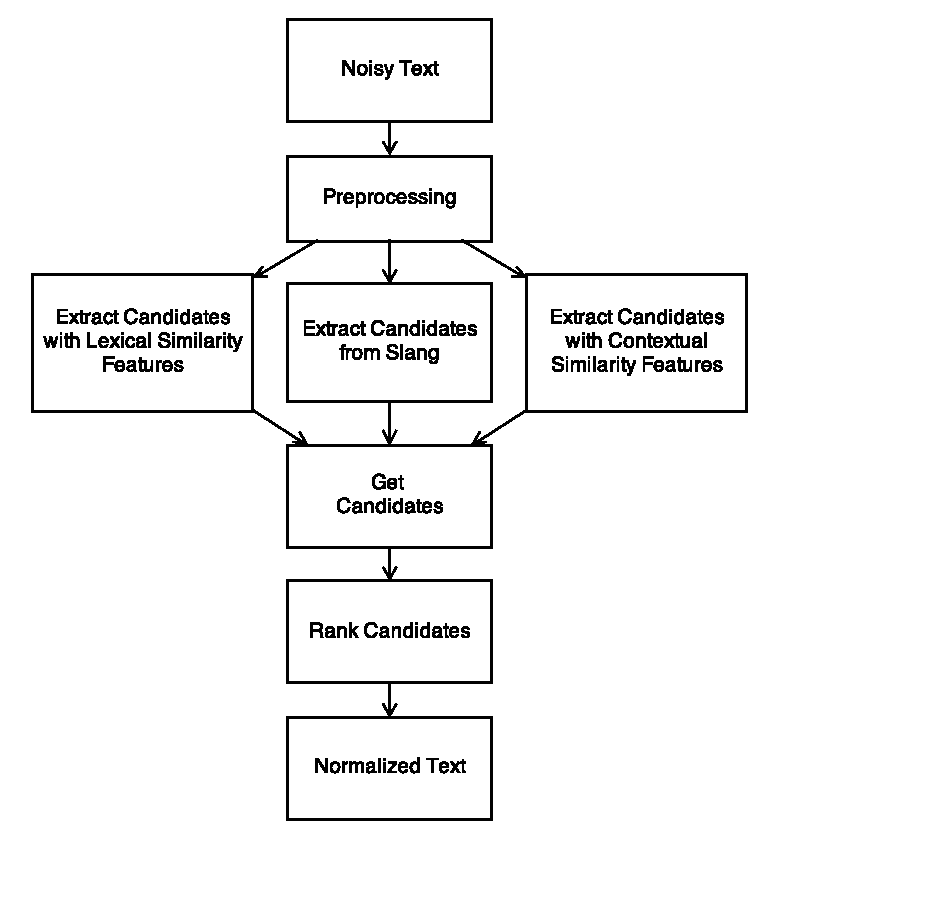
\includegraphics[scale=0.6]{fig/overview}
\caption{High level overview of our system}
\label{fig:overview}
\end{center}
\end{figure}

\subsection{Preprocessing}

%Tokenization is the first step in our system. Tokenization is the process of breaking the text into words, numbers, symbols, emoticons After tokenization, next in the pipeline is POS tagging each token using a social media POS tagger. Unlike the normal POS taggers, social media POS taggers~\cite{DBLP:conf/naacl/OwoputiODGSS13}\cite{Gimpel:2011:PTT:2002736.2002747} provide a broader set of tags that is special to the social text. By this extended set of tags we can identify tokens such as discourse markers~(rt for retweets, cont. for a tweet whose content follows up in the coming tweet) or URLs. So that we can process those tokens within their context.

Tokenization is the first step in our system. It is the process of breaking the text into tokens, which are the smallest meaningful elements such as numbers, symbols, and emoticons. After tokenization, the next step in the pipeline is Part-of-Speech (POS) tagging each token using a POS tagger specifically designed for social media text. Unlike the regular POS taggers designed for well-written newswire-like text, social media POS taggers provide a broader set of tags specific to the peculiarities of social text ~\cite{DBLP:conf/naacl/OwoputiODGSS13,Gimpel:2011:PTT:2002736.2002747}. Using this extended set of tags we can identify tokens such as discourse markers~(e.g. rt for retweets, cont. for a tweet whose content follows up in the coming tweet) or URLs. This enables us to better model the context of the words in social media text.

As shown in Table~\ref{tab:postags}, after preprocessing, each token is assigned a POS tag with a confidence measure between 0 and 1. Later, we use these confidence scores in calculating the edge weights in our context graph. Note that even though the words \emph{w} and\emph{ beatiful} are misspelled, they are tagged correctly by the tagger, with lower confidence scores though.

\begin{table}[htbp]
\begin{minipage}{.5\linewidth}
\begin{tabular}[h]{|llr|}
 \hline
Token & POS tag & Confidence \\
 \hline
with & P & 0.9963 \\
 \hline
a & D & 0.998 \\
 \hline
beautiful & A & 0.9971 \\
 \hline
smile & N & 0.9712 \\
 \hline
\end{tabular}
\end{minipage}
\begin{minipage}{.5\linewidth}
\begin{tabular}[h]{|llr|}
 \hline
Token & POS tag & Confidence \\
 \hline
w & P & 0.7486 \\
 \hline
a & D & 0.9920 \\
 \hline
beatiful & A & 0.9733 \\
 \hline
smile & N & 0.9806 \\
 \hline
\end{tabular}
\end{minipage}
\caption{Sample POS tagger output obtained by using CMU Ark Tagger (P:Pronoun, D:Determiner, A:Adjective, N:Noun, G:Miscellaneous)~\cite{DBLP:conf/naacl/OwoputiODGSS13,Gimpel:2011:PTT:2002736.2002747}}
\label{tab:postags}
\end{table}

\subsection{Graph construction}

Contextual information of words is modeled through a word association graph created by using a large corpus of social media text. The graph encodes the relative positions of the POS tagged words in the text with respect to each other. After preprocessing, each text message in the corpus is traversed in order to extract the nodes and the edges of the graph.
%The graph~(See Figure~\ref{fig:graph}) is build using a big dataset of social media text. After preprocessing, we traverse each entry in the dataset and extract nodes and edges.
A node is defined with four properties: \textit{id, oov, freq, tag}. The token itself and it's POS tag form the \textit{id} field. The \textit{freq} property indicates the node's frequency count in the dataset. The \textit{oov} field is set to True if the token is an OOV word. Following the prior work by Han and Baldwin, 2011 we used the GNU Aspell dictionary (v0.60.6) to determine whether a word is OOV or not~\cite{Han:2011:LNS:2002472.2002520}. Table~\ref{tab:graph} shows a sample tokenized and tagged sentence from the corpus, as well as the nodes and edges that are extracted from it to create the word association graph. A portion of the graph that covers this sample sentence is shown in Figure~\ref{fig:graph}.

\begin{table}[tbhp]
\begin{minipage}[c]{\linewidth}
\fxbox{
Let's$_{\textcolor{red}{L}}$ start$_{\textcolor{red}V}$ this$_{\textcolor{red}D}$ morning$_{\textcolor{red}N}$ w$_{\textcolor{red}P}$ a$_{\textcolor{red}D}$ beatiful$_{\textcolor{red}A}$ smile$_{\textcolor{red}N}$.$_{\textcolor{red},}$
 }\par
\vspace{5mm}
\end{minipage}
\begin{minipage}[c]{\linewidth}
\begin{tabular}[h]{l|l}
Tokens & Let's, start, this, morning, w, a, beatiful, smile,~. \\
\hline
Nodes & Let's$|$L, start$|$V, this$|$D, morning$|$N, w$|$P, a$|$D, beatiful$|$A, smile$|$N, .$|$, \\
\hline
Edges & \{Let's$|$L, start$|$V , distance:1\},\{Let's$|$L, this$|$D, distance:2\}, \\
& ... \\
& \{a$|$D, beatiful$|$A, distance:1\}, \{a$|$D, smile$|$N, distance:2\}, \\
& \{beatiful$|$A, smile$|$N, distance:1\} \\
\end{tabular}
\end{minipage}
\caption{Sample tokenized, POS tagged sentence and the corresponding nodes and edges in the word association graph.}
\label{tab:graph}
\end{table}

\begin{figure}[htb]
\begin{center}
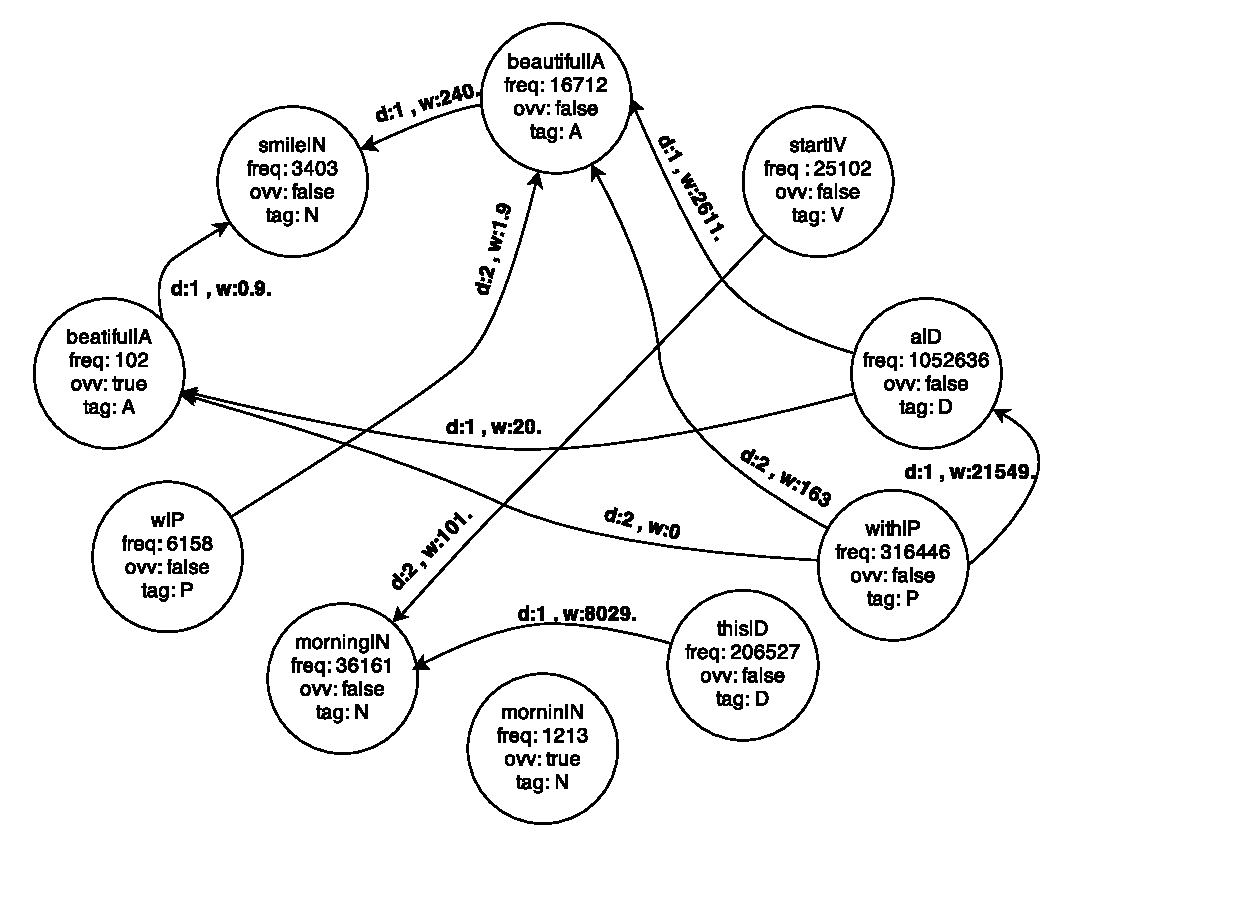
\includegraphics[scale=0.6]{fig/graph}
\caption{Sample nodes and edges from the word association graph.}
\label{fig:graph}
\end{center}
\end{figure}

%We define a node with four properties \textit{id, oov, freq, tag}. The token itself plus it's POS tag forms the \textit{id} field. \textit{freq} property indicates the node's frequency count in the dataset. \textit{oov} field is set to True if the token is a OOV word. Following ~\cite{Han:2011:LNS:2002472.2002520} we used GNU Aspell dictionary (v0.60.6) to determine whether a word is OOV or not.

%In the word-relatedness graph, each node is a unique set of a token and a POS tag (see Table~\ref{tab:graph}). This helps us to identify the tokens not only lexically and contextually but also (in terms of POS tags) grammatically.

In the created word association graph, each node is a unique set of a token and its POS tag. This helps us to identify the candidate IV words for a given OOV word by considering not only lexical and contextual similarity, but also grammatical similarity in terms of POS tags. For example if the token \textit{smile} has been frequently seen as a Noun or a Verb, and not in other forms in the dataset~(e.g. ~Table \ref{tab:nodes}), this provides evidence that it is not a good IV candidate as a normalization for an OOV token that has  been tagged as a Pronoun. On the other hand, \textit{smile} can be a good candidate for a Noun or a Verb OOV token, if it is lexically and contextually similar to it.

\begin{table}[hbt]
  \centering
  \begin{tabular}[tc]{l}
    node id : smile$|$A , freq : 3, oov : False, tag : A \\
    node id : smile$|$N , freq : 3403, oov : False, tag : N \\
    node id : smile$|$V , freq : 2796, oov : False, tag : V \\
  \end{tabular}
  \caption{The nodes in the word association graph representing the token \textit{smile} tagged with different POS tags.}
\label{tab:nodes}
\end{table}

An edge is created between two nodes in the graph, if the corresponding word pair (i.e. token/POS pair) are contextually associated. Two words are considered as contextually associated if they satisfy the following criteria:

\begin{itemize}
\item The two words co-occur within a maximum word distance of $d_t$ in a text message in the corpus.
\item Each word has a minimum frequency of $f_t$ in the corpus.
\end{itemize}

The directionality of the edges is based  on the sequence of words in the text messages in the corpus. In other words, an edge between two nodes is directed from the earlier seen token towards the later seen token. For example, Table~\ref{tab:edges} shows the edges that would be derived from a text including the phrase ``with a beautiful smile''. The \textit{from} property indicates the first word and \textit{to} is the latter in the phrase. The direction and the distance together represent a unique triplet. For each pair of nodes with a specific distance there is an edge with a positive weight, if the two nodes are related. Each co-occurrence of two related nodes increases the weight of the edge between them with an average of the nodes' POS tag confidence scores in the text message considered. If we are to expand the graph with the example phrase shown in Table~\ref{tab:edges}, the weight of the edge with distance $3$ from the node \emph{with$|$P}  to the node  \emph{smile$|$N} would increase by $(0.9963+0.9712)/2$, since the confidence score of the POS tag for the token \emph{with} is  $0.9963$ and the confidence score of the POS tag of the token \emph{smile} is $0.9712$ as shown in Table~\ref{tab:postags}.
%using the given POS tags and accuracies from Table~\ref{tab:postags}, the increase in the weights would be respectively $0.9963+0.9712/2$, $0.998+0.9712/2$ and %$0.9971+0.9712/2$.

\begin{table}[hbt]
  \centering
  \begin{tabular}[tc]{l}
 from : with$|$P, to : smile$|$N, dis : 3, weight : 72.24415 \\
 from : a$|$D, to : smile$|$N, dis : 2, weight : 274.37365 \\
 from : beautiful$|$A, to : smile$|$N, dis : 1, weight : 240.716 \\
\end{tabular}
  \caption{Example edges extracted from the sample phrase  ``with a beautiful smile''}
\label{tab:edges}
\end{table}


\subsection{Graph Based Contextual Similarity}

When we have an entry to normalize, next step after preprocessing is finding normalization candidates for each OOV token in the entry. For each ill-formed OOV token $t_i$ in a given entry, we first list the nodes that is related to $t_i$. The list includes all the nodes related to $t_i$ and their positional distance to the $t_i$ in the entry. We will refer to this list as neighbour list $NL_i$. In Table~\ref{tab:neigh} you can find a sample neighbour list for the OOV token beatiful$|$A from the sample sentence in Table~\ref{tab:graph}.

\begin{table}[hbt]
  \centering
  \begin{tabular}[tc]{l}
    w$|$P, position: -2 \\
    a$|$D, position: -1 \\
    smile$|$V, position: 1 \\
  \end{tabular}
\caption{Example neighbour list for the OOV node beatiful$|$A}
\label{tab:neigh}
\end{table}


For each neighbour node $n_{ij}$ in the $NL_i$  we traverse the graph and find the edges from or to the node ($n_{ij}$). The resulting edge list $EL_{ij}$ has edges in the form of ($n_{ij}$, candidate) or (candidate,$n_{ij}$) and includes all the nodes that are related to the node $n_{ij}$. Here the neighbour node can be an OOV node but the candidate node chosen among the IV nodes. We filter the edges in $EL_{ij}$ by the relative distance of $n_{ij}$ to the $t_i$ given in the $NL_i$. Each (neighbour, candidate) tuple should have the exact distance as the neighbour and OOV token has.

One last step is to conduct a POS tag filtering on the edges in $EL_{ij}$. Each candidate node should have the same POS tag with its OOV token. For the OOV token $t_i$ which has tag $T_i$, all the edges that include candidates with a tag other than $T_i$ are removed from the edge list $EL_{ij}$. Thus $EL_{i}$ contains edges only with $c_{ik}$s that is tagged with $T_i$.

Each edge in the $EL_{ij}$ has a neighbour node $n_{ij}$, a candidate node $c_{ik}$ and an edge weight $ew_{ijk}$. The edge weight, represents the likelihood or the degree of the relatedness between the the neighbour node $n_{ij}$ and candidate node $c_{ik}$(Eq~\ref{eq:ew}). Since we are looking for candidate nodes that is most likely to be the correct canonical form of the OOV word $t_i$, this metric is a good indicator. However, weight of the common phrases are much more higher than the average weight. That results in favouring the words with higher frequencies like stop words. To avoid this we normalize the edge weight $ew_{ijk}$ with the frequency of the neighbour node $n_{ij}$(See Eq~\ref{eq:ew_norm}).

\begin{equation}
ew(n,pos,c) =
\begin{cases}
  w : (n,c,distance = |pos|,weight=w), & \text{if } pos < 0 \\
  w : (c,n,distance = |pos|,weight=w), & \text{otherwise}
\end{cases}
\label{eq:ew}
\end{equation}

\begin{equation}
ewNormalized(n,pos,c) = ew(n,pos,c) / frequency(c)
\label{eq:ew_norm}
\end{equation}


We have a metric that assures contextual similarity based on binary relatedness. However we need more than binary relatedness to achive a comprehensive contextual coverage. To assure this broader coverage, one contextual similarity feature is built based on sum of the binary relatedness scores of several neighbours. For a candidate node $c_{ik}$ the total edge weight score is the sum of $ew_{ijk}$ which is the edge weights coming from different neighbours of the OOV token $t_i$. You can find the formula in Equation~\ref{eq:wscore}. We expect this contextual similarity feature to favour and XXX(find) the candidates which are (1)related to as many neighbours as possible and (2)have a high relatedness score with each neighbours.

\begin{equation}
edgeWeightScoreNeigh(t,n,c,pos) = \sum_{n,c \in EL(t,n)}{ewNormalized(n,pos,c)} \\\\
\end{equation}
\begin{equation}
edgeWeightScore(t,c) = \sum_{n,pos \in NL(t) }{contSimCostNeigh(t,n,c,pos)}
\label{eq:wscore}
\end{equation}

Since the graph includes both OOV and IV tokens and our OOV detection depends on the spellchecker which excepts some OOV tokens that has the same spelling with another IV word as IV, to be able to propose better canonical forms, the frequency of normalization candidates has been also added to the contextual similarity feature. Nodes with higher frequencies lead to tokens', that are in their most likely grammatical forms.

To calculate the final contextual similarity cost, we sum the total edge weight score and a frequency score between 0 and 1 (proportional to their frequency) (See Eq~\ref{eq:contscore}). Since the total edge weight score is our primary contextual resource, while calculating the total contextual similarity metric, we assigned to the frequency feature, only half weight of the total edge weight score.

\begin{equation}
contScore(t,c) = \lambda_a edgeWeightScore(t,c) + \frac{\lambda_a} 2 freqScore(c)
\label{eq:contscore}
\end{equation}

Hereby, we have the candidate list $CL_{i}$ for the OOV token $t_i$ that includes all the unique candidates in $EL_{i}$ and their contextual similarity costs calculated.

\subsection{Lexical Similarity}

Following~\cite{Han:2011:LNS:2002472.2002520,DBLP:conf/acl/HassanM13}, we built our lexical similarity features over standard edit distance~\cite{levenshtein1966bcc}, double metaphone(phonetic edit distance)~\cite{Philips:2000:DMS:349124.349132} and longest common subsequence ratio over edit distance(LCSR)~\cite{Contractor:2010:UCN:1944566.1944588}.

We calculated both edit distance, phonetic edit distance and LCSR of each candidate in $CL_{ij}$ and OOV token $t_i$.

Following the tradition that is inspired from~\cite{Kaufmann2010} before lexical similarity calculations any repetitions more than 3 letters in OOV tokens are reduced to 2. (gerci onlar 3e reduce etmis ama)

We used edit distance and phonetic edit distance to filter the candidates. Any candidate in $CL_{ij}$ with an edit distance greater than $ed_t$ and phonetic edit distance greater than $ped_t$ to $t_i$ has been removed from the candidate list $CL_{ij}$.

For the rest of the candidates we calculated the total lexical similarity score(Eq~\ref{eq:lexscore}) using LCSR and edit distance score~\footnote{an approximate string comparison measure (between 0.0 and 1.0) using the edit distance \url{https://sourceforge.net/projects/febrl/}}. Since the main lexical feature is LCSR, we applied the same distributions we used in contextual similarity score in calculating lexical score too.

\begin{equation}
lexScore(t,c) = \lambda_a LCSR(t,c) + \frac{\lambda_a} 2 editDistScore(t,c) + \lambda_a externalScore(t,c)
\label{eq:lexscore}
\end{equation}

Additionally, sistemin kısa entry'ler(context bağlantısı kurulamayacak kadar kısa), ve context'ten bağımsız token'ları da kapsayabilmesi için graph'ı tekrar dolaşıp contextual similarity feature'ı taşımasa da yukarıdaki filtreye uyuyorsa aday listesine ekledik.


son olarak external normalizasyonlar olarak slang dictionarydeki entryleri, sayıları ve pronounları externalScore veretek aday listesine ekliyoruz. externalScore binary bir feature 0 ya da 1.
\begin{verbatim}
units = ["", "one", "to", "three", "for",  "five", "six", "seven", "eight", "nine"]
pronouns = {u'2':u"to",u'w':u"with"}
\end{verbatim}


\begin{equation}
candScore(t,c) = lexScore(t,c) + contScore(t,c)
\label{eq:candscore}
\end{equation}

\section{Experiments}
\label{sec:experiments}

\subsection{Data set}
We used LexNorm1.1 dataset~\cite{Han:2011:LNS:2002472.2002520} to evaluate our approach. LexNorm1.1 contains 549 tweets with 1184 ill-formed OOV tokens.

\subsection{Graph Generation}
We used a large amount of social media text to construct our co-occurrence graph. We extracted 1.5GB English tweets from Stanford's 476 million Twitter Dataset~\cite{DBLP:conf/wsdm/YangL11}. The language identification of tweets is performed using the langid.py~\cite{Lui:2012:LOL:2390470.2390475, Baldwin:2010:LIL:1857999.1858026}.

After tokenization we removed tokens POS tagged as mention~(@brendon), discourse marker (ex: RT), URL, email addresses, emoticons, numerals and punctuations. Remaining tokens are used to build the graph.

For tokenization and POS tagging the tweets, we used CMU Ark Tweet Tagger~\cite{DBLP:conf/naacl/OwoputiODGSS13,Gimpel:2011:PTT:2002736.2002747}. Ark Tweet Tagger is a social media specific POS tagger and reported to perform $95\%$ accuracy over social media text.

The POS tagset of ark tagger includes some extra tags besides the standard part of speech tags that is specific to social media: URLs and emoticons; Twitter hashtags \#; twitter at-mentions (@). One other tag that is special to social media is \textasciitilde~means the token is specific to a discourse function of twitters. Lastly G stands for miscellaneous words including multi word abbreviations like btw~(by the way), nw~(no way), smh~(somehow).

We made use of this social media specific tags to disambiguate some OOV tokens. For example if OOV token ``cont'' is tagged with the discourse function tag G, we added ``continued'' to the candidate list as an external node.

After constructing the graph we only kept the nodes with a frequency greater than 8. For the performance related reasons, the relatedness thresholds $d_t$ and $f_t$  are chosen as 3 and 8 respectively. We had remaining 105428 nodes and 46609603 edges in the graph after the setup.

\subsection{Candidate Set Generation}

While extending the candidate set with lexical features we use ${ed_t \leq 2} \vee {ped_t \leq 1}$ to keep up with the settings in Han et al.~\cite{Han:2011:LNS:2002472.2002520}. IV words that is within 2 character edit distance of given OOV word or 1 character edit distance of given OOV word under phonemic transcription are chosen as lexical similarity candidates.

\subsection{Results and Analysis}

\begin{table}[thb]
  \centering
  \begin{tabular}[t]{lccc}
    \hline
    Method & Precision & Recall & F-measure \\
    \hline
    Han and Baldwin,2011 & 75.30 & 75.30 & 75.30 \\
    Liu et al.,2011 & 84.13 & 78.38 & 81.15 \\
    Hassan et al.,2013 & 85.37 & 56.40 & 69.93 \\
    Yang et al.,2013 & 82.09 & 82.09 & 82.09 \\
    CWA-Graph   & 86.20 & 78.0 & 82.0 \\
    \hline
  \end{tabular}
  \caption{Empirical Results produced on LexNorm1.1 dataset}
  \label{tab:results}
\end{table}

The results are presented in Table~\ref{tab:results}. Our system, Contextual Word Association Graph (CWA-Graph), achieved the highest precision among all other systems compared with the LexNorm1.1 dataset.

As well as precision, we managed to raise the F-Measure score without compromising much from the recall. Yet, we have the highest F-Measure score except the Yang et al.'s~\cite{DBLP:conf/wsdm/YangL11}.

The earlier work we compare our system with, assumes that the words to be normalized are given in advance. We also made the same assumption. However unlike other systems (\cite{DBLP:conf/wsdm/YangL11, liu2012broad, Han:2011:LNS:2002472.2002520}), our system may not propose a normalization, if there are no candidates that are lexically similar, grammatically correct and contextually close enough. For this reason we managed to achieve a higher recall compared to other systems. Besides, we make sure that the candidate has a minimum similarity either contextual, lexical, external or each. In Table~\ref{tab:thresholds} you can see how we reach higher degrees of precision by fine tuning the system threshold.

\begin{table}[thb]
  \centering
  \begin{tabular}[th]{lccc}
    \hline
    Threshold & Precision & Recall & F-measure \\
    \hline
    $\leq$ 1 & 81.40 & 81.1 & 81.20 \\
    1.1 & 84.40 & 79 & 81.60 \\
    1.2 & 87.90 & 76.30 & 81.7 \\
    1.3 & 84.80 & 79.50 & 82.00 \\
    1.4 & 85.40 & 79. & 81.90 \\
    1.45 & 86.20 & 78.1 & 82. \\
    1.6 & 90.00 & 72.1 & 80.10 \\
    1.7 & 92.50 & 68.9 & 79.00 \\
    1.8 & 94.50 & 60.4 & 73.70 \\
    \hline
  \end{tabular}
  \caption{Comparison of results for different threshold values, which set as at least $\lambda_a$}
\label{tab:thresholds}
\end{table}

\section{Conclusion}


%% The Appendices part is started with the command \appendix;
%% appendix sections are then done as normal sections
%% \appendix

%% \section{}
%% \label{}

%% References
%%
%% Following citation commands can be used in the body text:
%% Usage of \cite is as follows:
%%   \cite{key}          ==>>  [#]
%%   \cite[chap. 2]{key} ==>>  [#, chap. 2]
%%   \citet{key}         ==>>  Author [#]

%% References with bibTeX database:
\bibliographystyle{model1-num-names}
\bibliography{sentic}
\end{document}

%%
%% End of file `norm.tex'.
